% 

\documentclass[ai15_group61_report.tex]{subfiles}
\begin{document}

\subsection{Models used in experiment}
The models used in the experiments, we later realized, were implemented in a way that was inconsistent with the specifications outlined in {Inferred grammar model}. This was a big setback, since it effectively meant that the data gathered from the experiment told us nothing about the hypothetical models outlined in {Our method}.

We will use SM* and IGM* to refer to the implementation of the Semantic model and Inferred grammar model used in the experiment.

\subsubsection{Semantic model}
The Semantic model was inconsistent with the specifications in that it 


\subsubsection{Inferred grammar model}
The implementation of the Inferred grammar model (IGM*) was, among the two experimental models, the one most inconsistent with the specifications. 

IGM* separated grammar and words into two models which were used in sequence to generate text. The grammar model modeled trigrams of POS-tags, which was consistent with our specifications. The word-grammar model generated a new word, given the previous two POS-tags. This is inconsistent with the specifications. IGM* would take ``the man walked'' and create the trigrams (DET, NOUN, VERB) for the grammar model, and (DET, NOUN, walked) for the grammar-word model.

To highlight the inconsistency, IGM generates $(w_3|w_1,w_2,t_3)$, while IGM* generates $(w_3 | t_1,t_2)$.


\subsection{Experimental setup}
\label{sec:expiremental_setup}
Model performances were measured using a perception test in the form of an online survey with 30 questions. Both models were used to generate 3 sentences for each of the 4 smoothing methods.  Additionally 3 sentences were hand-picked from the Brown corpus and 3 sequences of random words generated to serve as the ``human'' and ``baseline'' models against which our models would be compared. Each group of 3 was picked by generating a few hundred sentences and picking the top 3 with the best perplexity score. The number of sentences was limited to 30 because in test trials a higher number resulted in participants not having the patience to finish. 

Participants were asked to rate on a scale of 1-5 how closely they felt the sentences resembled human writing. As a guideline they were told that if a sentence appeared to be random words it might receive a 1, if it showed some signs of coherence it might receive a 3, and if it looked like a person wrote it then it would receive a 5. To make the test as fair as possible the sentences were presented to each participant in a random order. 

The survey platform used was Google Forms and the results where pulled into R for processing and graphical representation.

\subsection{Results}
\label{sec:results}
The results for the two implemented models were very different. The density distribution of answers can been seen in figure~\ref{fig:hist1} which shows that the results for the Semantic Model are rather evenly spread while the results for Inferred Grammar Model are are very skewed with most scores very low. Looking at the performance of different smoothing methods in figure~\ref{fig:hist2} we see that the Semantic Model  

\begin{figure}
  \centering
    \subfloat[Performance of each model as well as the real and baseline sentences]    
    {{\label{fig:hist1}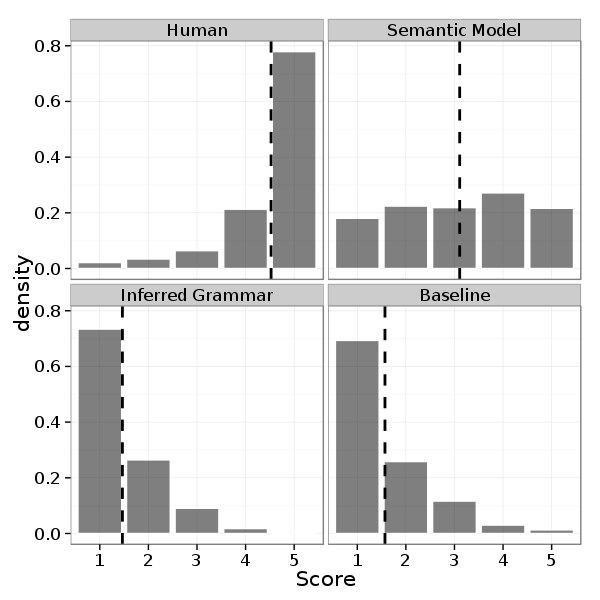
\includegraphics[height=5cm]{results/histogram_resultsByModel} 
    }}%
    \qquad
    \subfloat[Performance of each model and smoothing method]{{\label{fig:hist2}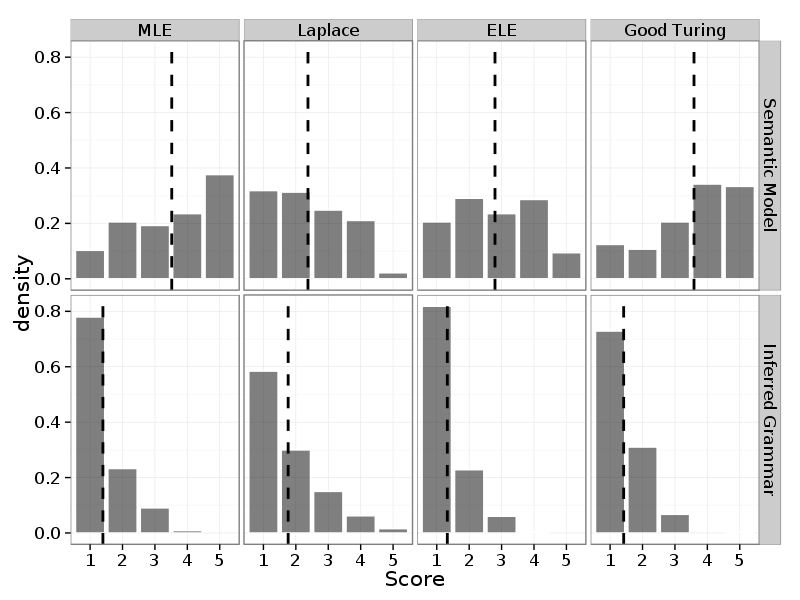
\includegraphics[height=5cm]{results/histogram_resultsByModelAndSmootingMethod} 
    }}%
    \caption{Density histograms of model performance in the perception test. Dotted lines represent means.}%
    \label{fig:histograms}%
\end{figure}

\begin{figure}%
    \centering
    \subfloat[Performance of each model as well as the real and baseline sentences]{{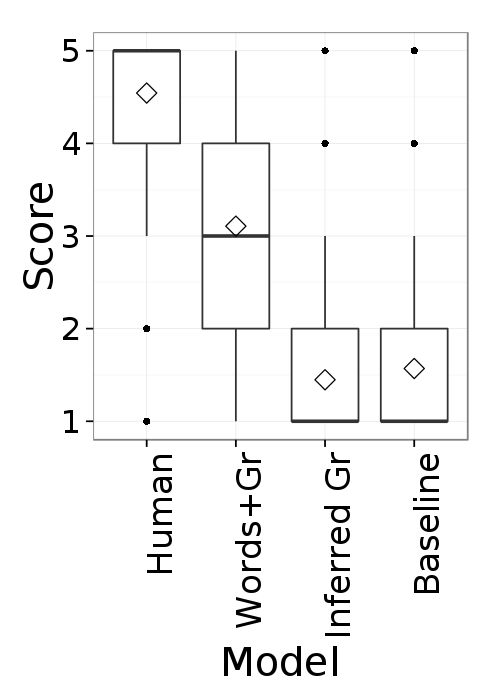
\includegraphics[height=6.2cm]{results/boxplot_resultsByModel} }}%    
    \qquad
    \subfloat[Performance of each model and smoothing method]{{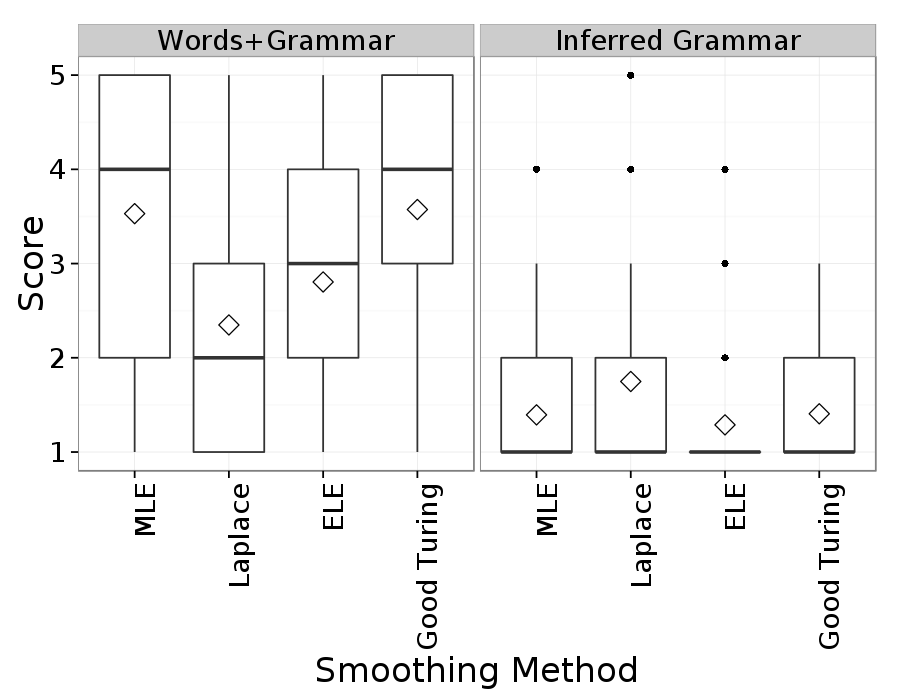
\includegraphics[height=6cm]{results/boxplot_resultsByModelAndSmoothing} }}%
    \qquad
    \caption{Boxplots of model performance in the perception test. Diamonds represent   means.}%
  \label{fig:boxplots}
\end{figure}



Here we talk about how which smoothing technique worked best for us why the results were the way they were. We also explain why the model containing the grammar was better than the inferred grammar one.

\begin{figure}
\centering
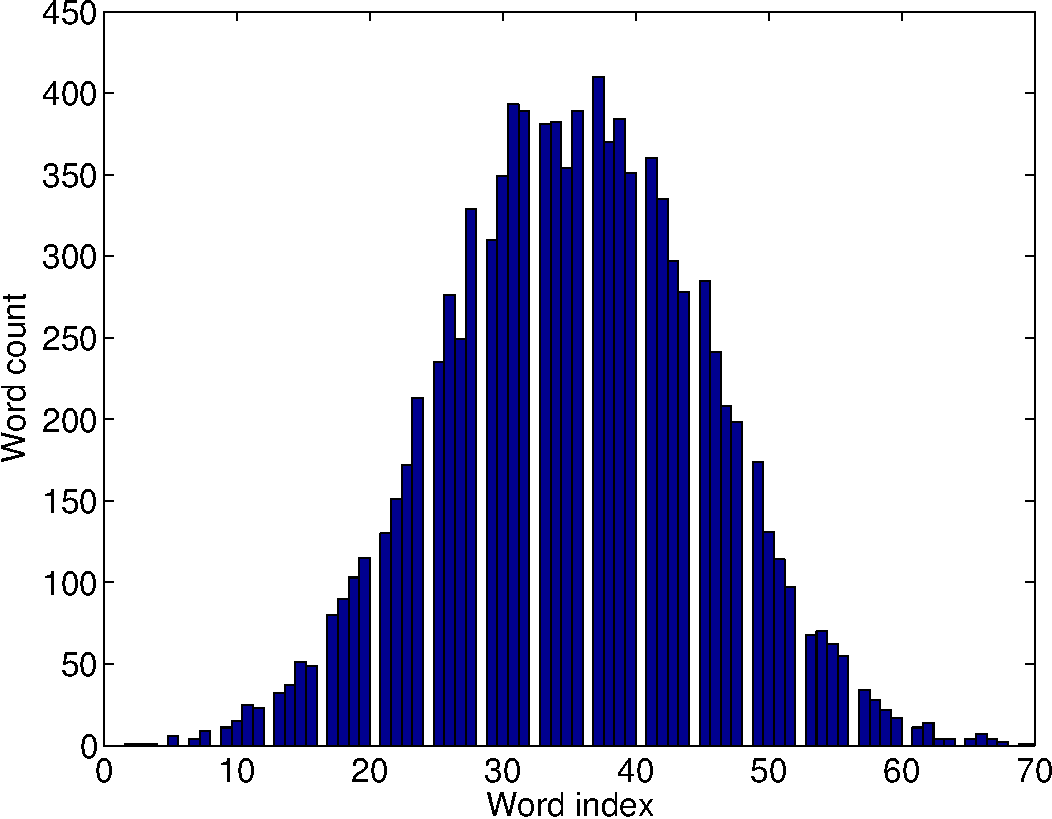
\includegraphics[width=0.8\linewidth]{histogram}
\caption{A description that makes browsing the paper easy and clearly
describes what is in the picture. Make sure that the text in the figure
is large enough to read and that the axes are labelled.}
\label{fig:histogram}
\end{figure}



\begin{table}
\begin{center}
\begin{tabular}{|c|c|c|}
\hline
Bla bla & Bla bla & Bla bla \\ \hline
42 & 42 & 42 \\ \hline
42 & 42 & 42 \\ \hline
\end{tabular}
\caption{A description that makes browsing the paper easy and clearly
describes what is in the table.}
\label{tab:results}
\end{center}
\end{table}

What answer was found to the research question; what did the study find? Was the tested hypothesis true?

%%%%%%%%%%%%%%%%%%%%%%%%%%%%%%%%%%%%%%%%%%%%%%%%%%%%%%%%%%%%%
%%%%%%%%%%%%%%%%%%%%%%%%%%%%%%%%%%%%%%%%%%%%%%%%%%%%%%%%%%%%%


\end{document}